
\section{Solr}

Der erste Kandidat ist Solr. Der Download ist direkt auf der Website ohne Registrierung zu finden. \cite{TheApacheSoftwareFoundation.2019}. Da Solr komplett Open Source ist, kann sich neben den Binary’s auch der Source-Code heruntergeladen werden. 

\subsection{Installation}

Als Systemvoraussetzungen ist eine Java Version $> 8$ gegeben. Ich habe mich hierbei für OpenJDK 11 entschieden. 
Nach dem ersten Starten wurden 2 Warnungen gemeldet, dass gewisse Limits zu gering für Solr sind \ref{lst:warningSolr}. Nachdem beide entsprechend erhöht wurden, verschwanden die Warnungen.

Die Development-Installation ist denkbar einfach. Zuerst wird Solr aus dem Archiv entpackt und dann mit \path{bin/solr start} gestartet. Hierbei wurde ich allerdings direkt von 2 Warnungen begrüßt. 

\begin{lstlisting}[language=bash, frame=single, label={lst:warningSolr}] 
    *** [WARN] *** Your open file limit is currently 1024.
    It should be set to 65000 to avoid operational disruption.

    *** [WARN] ***  Your Max Processes Limit is currently 63918.
    It should be set to 65000 to avoid operational disruption.
\end{lstlisting}

Die richtige Installation installiert Solr als Service und legt sich einen Nutzer an. Ein entsprechendes Installations-Skript findet sich dafür im entpackten Solr-Ordner.

\subsection{Indexierung}

Um mit der Indexierung starten zu können, muss zuerst in sogenannter „Core“ erstellt werden. Dieser ist ein Index mit dazugehörigen Transaktionslog und Konfigurationsdateien. Nur mit diesen ist es möglich Dateien zu indexieren und auf ihnen zu suchen. Nach der Erstellung lässt sich der Core nun auch über die Oberfläche einsehen und zum Teil konfigurieren.

Damit Solr nun die Daten von der Datenbank liest, muss ein DataImportHandler (DIH) \ref{lst:dih} geschrieben werden. In diesen werden die Daten, welche Indexiert werden sollen mit MySQL-Queries eingelesen. Das System basiert dabei auf Entitys. Diese Entitys besizten jedeweils mehre Attribute, wie den Name, welcher auf der Oberfläche zur Indexierung angezeigt wird, den MySQL von dem die Daten geladen werden und einen Delta-Query, welcher nur die neuen Einträge lädt. Der Delta-Query benötigt hierbei eine eigene Spalte in der Datenbank, die einen Timestamp besitzt, der angezeigt, wann die Spalte das letzte mal editiert wurde. Da die Tabellen, diese Spalte aktuell nicht besitzen, wird der Delta-Query nicht getestet werden können. Innerhalb des Entity Elements gibt es entweder weitere Entitys, dazu gleich mehr, oder Field-Elemente. Diese besitzen ein Attribut, welches die Spalte der Tabelle ausweist und einen Namen, der das zugehörige Solr-Schema-Element ausweist. Entitys können unbegrenzt ineinander verschachtelt werden. Damit Änderungen an einer verschachtelten Entity nach oben richtig weitergegeben werden, gibt es ParentDeltaQuerys. Diese geben die betroffenen Werte an die übergeordnete Entity weiter. Dafür führt der ParentDeltaQuery einen Aufruf an die überliegende Entity-Tabelle aus in der er mithilfe der Femdschlüssel-Ids in den betroffen Zeilen herausfindet.

\begin{lstlisting}[language=xml, frame=single, label={lst:dih}, 
    morekeywords={entity,query,deltaQuery,parentDeltaQuery,field,column, name}] 
    <entity name="tfl_fehler" 
            query="select * from tfl_fehler" 
            deltaQuery="select eid from tfl_fehler 
                where last_modified > '${dataimporter.last_index_time}'"> 

		<field column="originalText" name="originalText" />
		<field column="band" name="band" />
        [...] <!-- more Columns -->

      <entity name="tfl_fehler_rptmap"
              query="select fk_rptmap from tfl_fehler_rptmap 
                where fk_fehler='${tfl_fehler.eid}'"
              deltaQuery="select fk_rptmap, fk_fehler 
                from tfl_fehler_rptmap 
                where last_modified > '${dataimporter.last_index_time}'"
              parentDeltaQuery="select eid from tfl_fehler
                where eid=${tfl_fehler_rptmap.fk_fehler}">

        <entity name="tfl_rptmap" [...]> <!-- Queries for rpt_map -->
          <field column="description" name="description" />
        </entity>
      </entity>
    </entity>
\end{lstlisting}

Wie schon eben angesprochen, muss das Solr-Schema für die entsprechende Elemente auch angepasst werden. Dafür gibt es diverse Möglichkeiten, zum einen kann eine XML-Datei angelegt werden, in welcher genau beschrieben wird, wie die einzelnen Einträge indexiert werden sollen. Diese Methode soll allerdings nicht mehr verwendet werden, da es die Möglichkeit gibt, diese Einträge per API einlesen zu lassen. Dabei wird direkt überprüft, ob die Einträge formal stimmen, so können keine fehlerhaften Schema gebaut werden. Dabei werden die Einträge dann in einen Managed Schema gespeichert. 

\begin{lstlisting}[language=xml, frame=single, label={lst:dih}, 
    morekeywords={entity,query,deltaQuery,parentDeltaQuery,field,column, name}] 
    <entity name="tfl_fehler" 
            query="select * from tfl_fehler" 
            deltaQuery="select eid from tfl_fehler 
                where last_modified > '${dataimporter.last_index_time}'"> 

		<field column="originalText" name="originalText" />
		<field column="band" name="band" />
        [...] <!-- more Columns -->

      <entity name="tfl_fehler_rptmap"
              query="select fk_rptmap from tfl_fehler_rptmap 
                where fk_fehler='${tfl_fehler.eid}'"
              deltaQuery="select fk_rptmap, fk_fehler 
                from tfl_fehler_rptmap 
                where last_modified > '${dataimporter.last_index_time}'"
              parentDeltaQuery="select eid from tfl_fehler
                where eid=${tfl_fehler_rptmap.fk_fehler}">

        <entity name="tfl_rptmap" [...]> <!-- Queries for rpt_map -->
          <field column="description" name="description" />
        </entity>
      </entity>
    </entity>
\end{lstlisting}

Dieser muss dann jedoch noch mit dem Core verbunden werden, dafür wird er, zusammen mit einem JDBC-Treiber in die solrconfig.xml eingetragen. Bei den JDBC-Treiber habe ich mich für dieses Beispiel für den Treiber von MariaDB entschieden. Damit es nicht deswegen zu Laufzeit-Unterschieden bei der Indexierung kommen kann, werde ich diesen Treiber bei allen Systeme mit JDBC-DataImportHandlern verwenden.

Als ich den Crawler allerdings startete, meldet mir Solr, das wenige Einträge indexiert wurden. Bei genauerer Betrachtung fand ich heraus, dass nur eine Tabelle von Solr betrachtet wurde. Als ich mir nun die Daten dieser Tabelle herausgegeben habe, bemerkte ich, dass nur das Feld „id“ indexiert wurde. Dies liegt daran, dass nur Felder in den Solr-Index geschrieben werden, die vorher im Schema festgelegt wurden. Dieses Schema kann man entweder über die Weboberfläche oder die API geändert werden kann. Es gibt auch eine Möglichkeit, das Schema direkt zu ändern, allerdings ist diese Methode nicht mehr erwünscht, da die API Fehler erkennt und Einträge so direkt ablehnt. Die so eingelesen Einträge werden in einem sogenannten Managed-Schema \ref{lst:managedSchema} gespeichert. Dort kann man einstellen, wie genau der Eintrag indexiert werden soll. Dabei können viele Einstellungen getroffen werden, um die beste Geschwindigkeit zu garantieren. Für diesen Test wurden die Grundeinstellungen verwendet. Bei der späteren richtigen Implementierung wird auf die einzelnen Felder nochmals genauer eingegangen. {LINK EINFÜGEN GENAUERE DATEN!!!} Aktuell möchte ich nur darauf eingehen, dass man mit "multiValued" eine Einstellung treffen kann, die es erlaubt 1 zu N Beziehungen abzubilden. Zusammen mit der Verschachtelung können so auch M zu N Verbindungen abgebildet werden. 

\begin{lstlisting}[language=xml, frame=single, label={lst:managedSchema}, 
    morekeywords={type,uninvertible,indexed,stored,field,multiValued, name}] 

    [...]
    <field name="ddc_webdewey_is_checked" type="boolean" 
        uninvertible="false" indexed="true" stored="true"/>
    <field name="description" type="text_de" uninvertible="false" 
        multiValued="true" indexed="true" stored="true"/>
    <field name="erweiterung" type="text_de" 
        uninvertible="false" indexed="true" stored="true"/>
    [...]

\end{lstlisting}

Die Indexierung lief eine Minute und 34 Sekunden für 14 Tausend Einträge \ref{img:solrIndexTime}. Dabei wurde der gegebene Arbeitsspeicher nicht komplett ausgenutzt, was schließen lässt, dass die Datenbank der limitierende Faktor war. Es wurden über 435 Tausend Aufrufe gegen die Datenbank gefahren, was darauf zurück zu führen ist, dass Solr keine Joins verwendet, sondern die Datenbank einfach für jede verschachtelte Entity nochmals durchläuft.

\begin{figure}
	\centering
	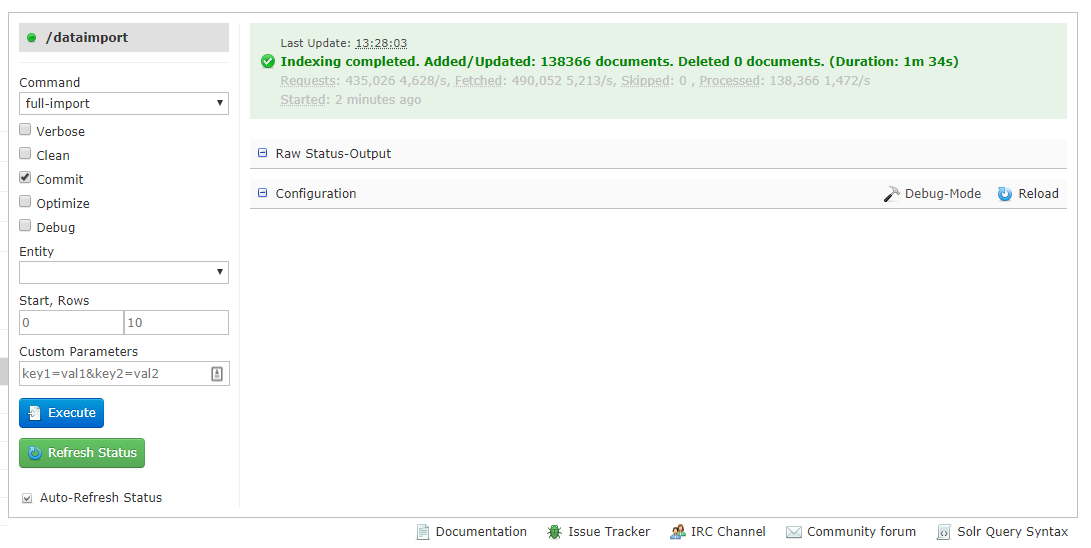
\includegraphics[width=1\linewidth]{images/solr_indexing_time.png}
	\caption{Startseite der Weboberfläche von Solr.}
	\label{img:solrIndexTime}
\end{figure}

\subsection{Oberfläche}

Der Startseite des Solr-Systems bietet direkten Einblick in auf die Auslastung des Systems. Der Fehler-Log ist auch sehr einfach mit einem Klick zu erreichen. Um Statistiken zu dem aktuellen Core zu bekommen, kann dieser aus einen Drop-Down-Menu einfach ausgewählt werden. Positiv anzumerken ist, dass es möglich ist das Schema direkt in der Weboberfläche zu modifizieren. Leider ist es nicht möglich, den DataImportHandler direkt zu verändern, ohne weitere Einstellungen im System vorzunehmen. Es gibt eine Möglichkeit Querys direkt über den Web-Client zu senden. Auch ist es möglich einen Debug-Modus bei den Query und den DataImportHandler einzuschalten. \ref{img:solrIndexTime} Auch können die Config-Dateien direkt im Browser angeschaut werden. Eine Editierung ist allerdings nicht möglich.
Es gibt keine Möglichkeit Updates direkt über die Weboberfläche einzuspielen, zudem ist die Seite auch nicht responsive geschrieben. 

\begin{figure}
	\centering
	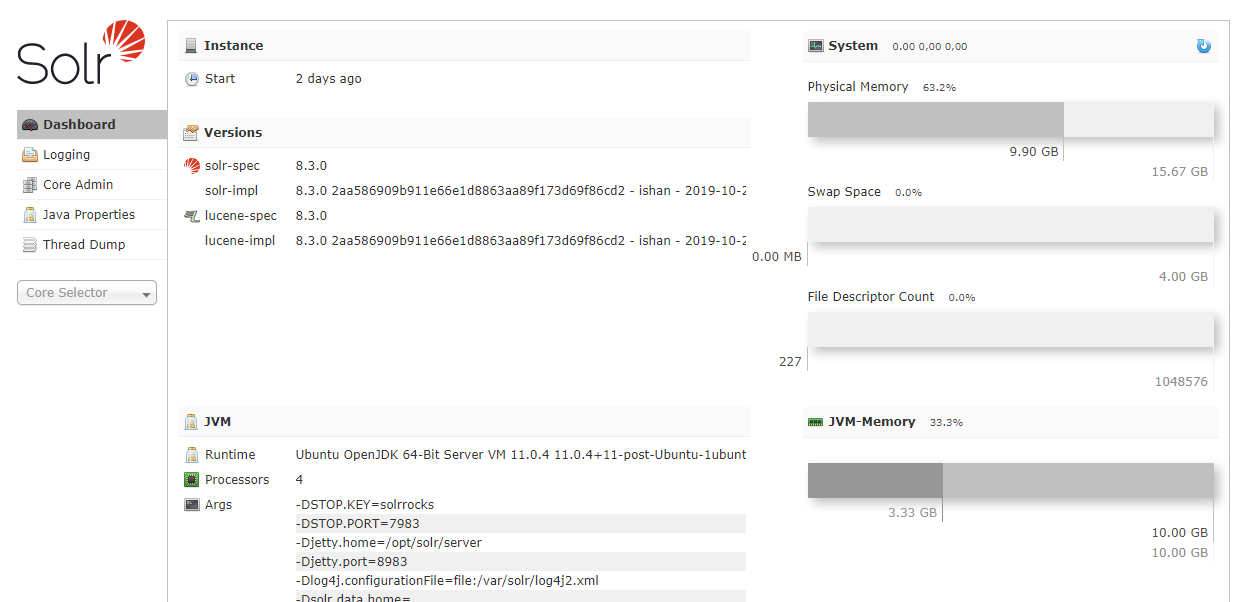
\includegraphics[width=1\linewidth]{images/solr_interface.png}
	\caption{Startseite der Weboberfläche von Solr.}
	\label{img:solrInterface}
\end{figure}


\subsection{Dokumentation}

Die Dokumentation war beim Setup meine Hauptquelle, die Installtion ist sehr genau beschrieben und auch die Systemanforderungen wurden genau beschrieben. Es gibt zu allen Attributen Erklärungen. Allerdings wäre ein Verweis, dass für die DataImportHandler-Attribute noch extra ein Solr-Schema-Attribut benötigt wird, schön gewesen. Dies habe ich erst durch einen Blog \cite{IqubalMustafaKaki.2016} herausgefunden und verstanden. Generell sollte die Dokumentation allerdings zu Administration ausreichen. 

\subsection{Absetzen einer Anfrage und Integration in PHP}

Um den Solr-Client in PHP nutzen zu können muss eine Erweiterung installiert werden. \cite{ThePHPGroup.2019}